\documentclass[a4paper,10pt]{jsarticle}
\renewcommand{\figurename}{Fig.}
\renewcommand{\tablename}{Table }
\usepackage[left=2cm,right=2cm,top=3cm,bottom=3cm]{geometry}
\usepackage{multicol}
\usepackage{blindtext}
\usepackage{amsmath,amsfonts}
\usepackage{bm}
\usepackage{siunitx}
\usepackage[dvipdfmx]{graphicx}
\usepackage{booktabs}
\usepackage{multirow}
\usepackage{here}
\usepackage{wrapfig}
\usepackage{siunitx}
\setlength{\columnsep}{10mm}
\makeatletter
\newenvironment{tablehere}
{\def\@captype{table}}
{}
\newenvironment{figurehere}
{\def\@captype{figure}}
{}
\makeatother

\begin{document}
\title{{等価回路の等価電圧測定における計器の内部抵抗の影響と\\テブナンの定理による解析値と実測値の比較}}
\author{Teduka Yuuki 1522063 
\\
Collaborator:Nakamura Kouta 1522B02 }
\date{Lab date: September 26th and October 3rd, 2023}
\maketitle

\begin{abstract}
  この実験の第一の目的は、等価回路の等価電圧を測定する際に、測定系(計器)の内部抵抗が及ぼす影響を調べ、被測定系の等価抵抗が十分大きくなった場合でも等価電圧を正確に測定できる計器を求めることである。
  特に、可動コイル型電圧計、エレクトロニクス電圧計、電位差計の3つの計器に焦点を当てて、それぞれの計器の内部抵抗が等価電圧の測定に与える影響を調べた。
  実験では、被測定系の等価回路の等価電圧と等価抵抗を既知とした状態で、等価抵抗を50Ωから100MΩまで変化させながら、開放端電圧を測定した。
  実験結果は、電位差計を用いた場合が最も安定して等価電圧に近い値を測定できることがわかった。一方、エレクトロニクス電圧計は可動コイル型電圧計と比べて内部抵抗が大きかったため、等価抵抗が100kΩ程度までならば安定して等価電圧を測定できることが示された。
  第二の目的は、与えられた複雑な直列回路網モデルにテブナンの定理を用いて解析し、テブナンの定理のよる解析値と実測値が一致することを確認することである。
  実験では、テブナンの定理を用いて等価回路の等価電圧と等価抵抗を求め、実測値と比較した。結果、有効数字2桁で一致した。
  さらに、電圧計の内部抵抗$R_m$を変化させた場合の開放端電圧を測定し、テブナンの定理で計算した理論曲線上に、実測値がプロットすることも確認した。

\end{abstract}

\begin{multicols}{2}
\section{Introduction}
図1のような、テブナンの定理の等価回路の等価電圧$E_{eq}$を測定する際、被測定系の内部抵抗$R_m$の影響を考慮する必要がある。実験では、3つの計器に焦点を当てて、それぞれの計器の内部抵抗が等価電圧の測定に与える影響を調べた。
具体的には、可動コイル型電圧計、エレクトロニクス電圧計、電位差計の3つの計器を用いて、テブナンの等価回路の等価電圧$E_{eq}$と等価抵抗$R_{eq}$を既知とした状態で、開放端電圧$V$を測定し、それぞれの計器の内部抵抗$R_m$を求め、計器の内部抵抗と等価抵抗の関係に基づいて、正確な等価電圧測定のための適切な計器の選択を明らかにした。等価電圧の正確な測定を行うための計器の選択基準を明らかにすることを目的としている。

以下、実験で扱った3つの計器について説明する。
\subsection{可動コイル型電圧計}
図1のような直流回路において、端子間A,Bの等価電圧$E_{eq}$を測定することを考える。\\

\begin{figurehere}
  \centering
  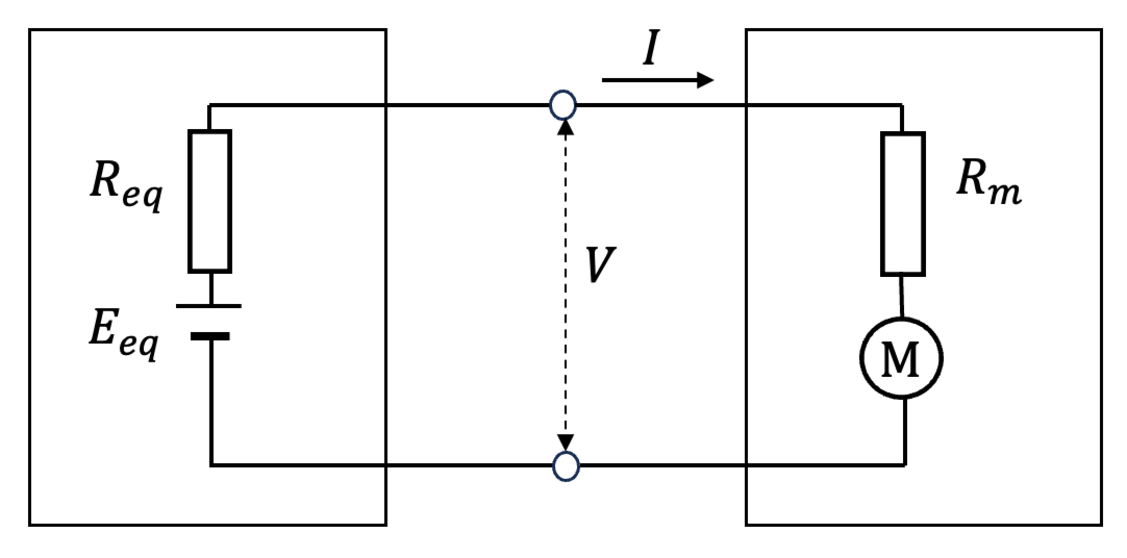
\includegraphics[width=0.8\linewidth]{figs/Equivalent_circuit_of_moving-coil_VM.pdf}
  \caption{Equivalent circuit of the measurement system under test and a movable coil voltmeter}
  \label{fig:equivalent_circuit}
\end{figurehere}

被測定系の電源電圧$E_{eq}$、抵抗$R_{eq}$、および可動コイル型電圧計の内部抵抗$R_m$が接続されている場合、回路に流れる電流$I$は:
\begin{equation}
I=\frac{E_{eq}}{R_{eq}+R_m}
\end{equation}
となる。
よって、$R_{eq}$による電圧降下$V_{R_{eq}}$は:
\begin{equation}
V_{R_{eq}}=IR_{eq}=\frac{E_{eq}R_{eq}}{R_{eq}+R_m}
\end{equation}
で計算されるから、端子間の電圧$V$は:
\begin{equation}
V=E_{eq}-V_{R_{eq}}=\frac{E_{eq}R_m}{R_{eq}+R_m}
\end{equation}
で測定される。従って、測定系の内部抵抗$R_m$の影響を小さくするためには、$R_m$の値を大きくする必要がある。\\
具体的には、$R_m$が$R_{eq}$に比べて十分大きい場合、測定される電圧$V$は電源電圧$E_{eq}$に非常に近くなる。
しかしながら、可動コイル型電圧計の場合、メーターMを動かすのにある程度の電流が必要になる。従って、$R_m$は十分に大きくすることができない。
\subsection{エレクトロニクス電圧計}
では、可動コイル型電圧計において、電流を小さくすることなく、$R_m$を大きくする方法はないだろうか。
可動コイル型電圧計の前に、図2のような電圧増幅器を接続することを考える。\\

\begin{figurehere}
  \centering
  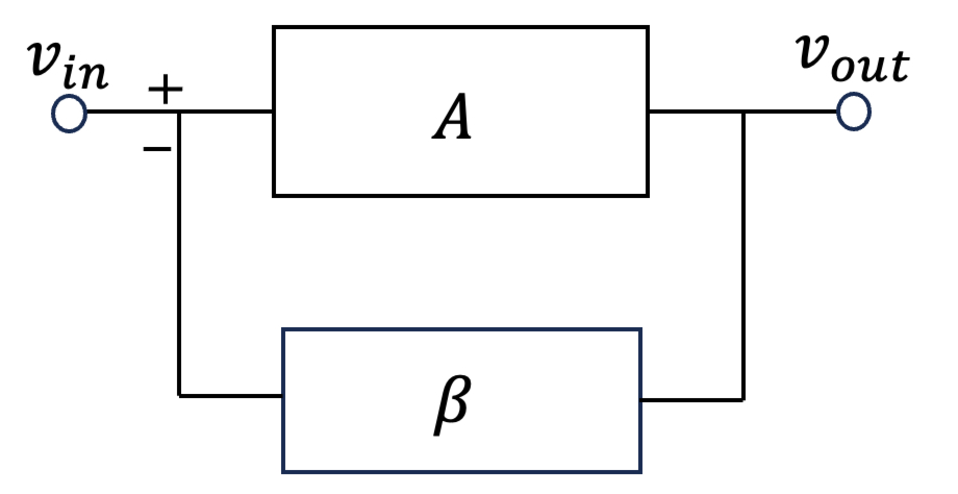
\includegraphics[width=0.6\linewidth]{figs/feedback.pdf}
  \caption{Feedback circuit}
  \label{fig:feedback}
\end{figurehere}


まず、入力電圧$v_{in}$は、電圧増幅度$A$を持つ増幅器によって増幅される。次に、増幅された電圧$v_{in}A$は、電圧増幅度$-\beta$のフィードバックを受ける。このフィードバックが無限回繰り返されることを考えると、出力電圧$v_{out}$は:
\begin{align*}
v_{out} &= v_{in}A + v_{in}A(-\beta A) + v_{in}A(-\beta A)^2 + \cdots \\
&= \frac{v_{in}A}{1+\beta A} 
\end{align*}
へと減少する。この電圧負帰還により、可動コイル型電圧計の内部抵抗$R_m$は、$R_m(1+\beta A)$へと増加する。このような電圧計をエレクトロニクス電圧計と呼ぶ。
\subsection{電位差計}
(2)式を見ると、電流$I = 0$の状態で電圧$V$を測ることができたら、$R_{eq}$の値によらず、$V_{R_{eq}}$の影響を小さくできる。
図3のように、検流計を見ながら電圧$V$を測定することを考える。\\
電流$I$が流れていないように、$V_{var}$を調整すると、電圧$V_2 = V = E_{eq}$となり、測りたい電圧$E_{eq}$を測定することができる。\\
\begin{figure}[H]
  \centering
  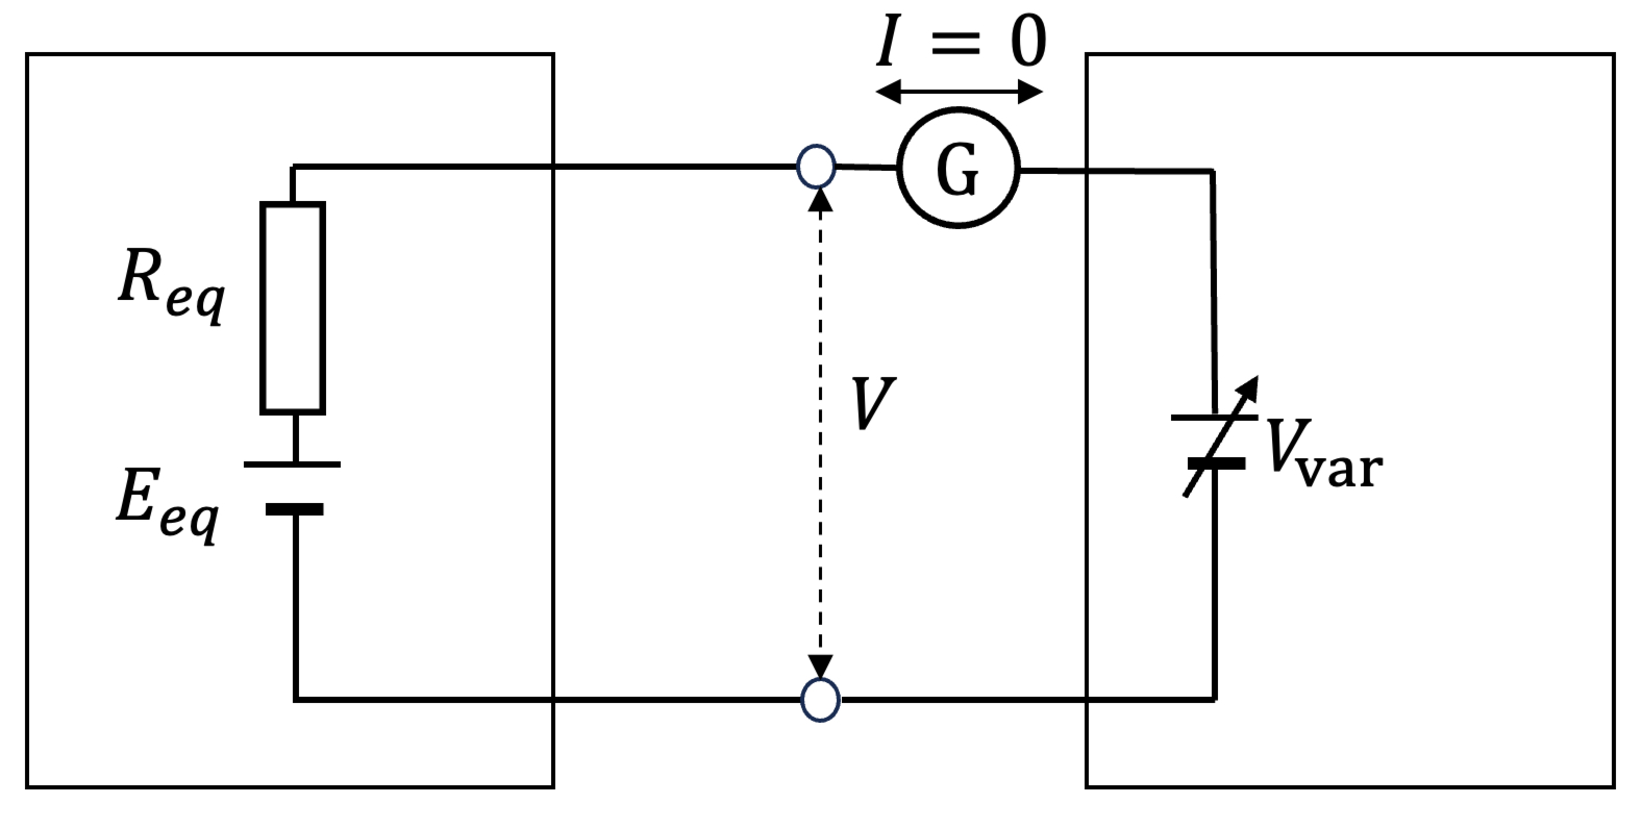
\includegraphics[width=0.8\linewidth]{figs/potentiometer.pdf}
  \caption{Diagram of potentiometer circuit}
  \label{fig:my_label}
\end{figure}
\section{Method}
まずは、可動コイル型電圧計、エレクトロニクス電圧計、電位差計の3つの計器を用いて開放端電圧を測定した。等価抵抗を50Ωから100MΩまで十分に大きくした場合の、等価電圧とのずれを調べた。
次に、テブナンの定理を検証するための実験を行った。
\subsection{開放端電圧の測定}
まず、測定系の回路図を図4に示す。
\begin{figure}[H]
  \centering
  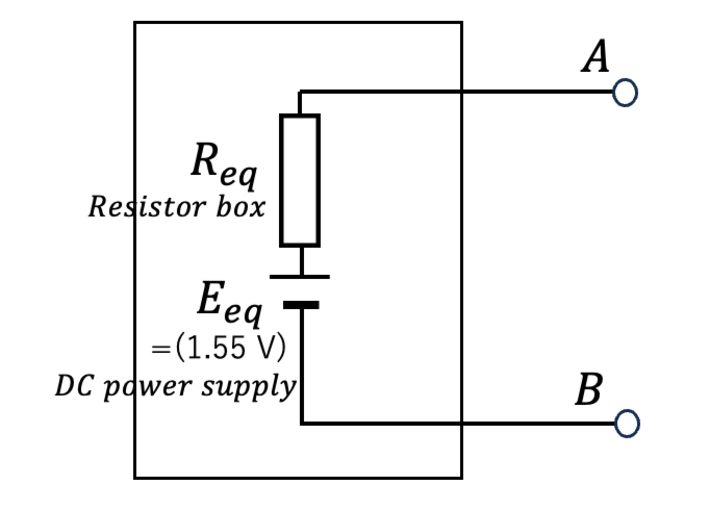
\includegraphics[width=0.8\linewidth]{figs/measuring_instrument.pdf}
  \caption{Circuit of the system under test}
  \label{fig:measuring_instrument}
\end{figure}
等価電圧$E_{eq}$は$1.550$Vで一定とし、$E_{eq}$の値は、測定が終わるまで変更しない。
等価抵抗$R_{eq}$は、抵抗箱を用いて、50 $\Omega$から100M $\Omega$まで変化させる。
その時の、端子A、B間の開放端電圧$E_{eq}$を、可動コイル型電圧計、エレクトロニクス電圧計、電位差計の3つの計器を用いて測定する。\\
電位差計を用いる場合の、回路図は図5に示した。\\
\begin{figure}[H]
  \centering
  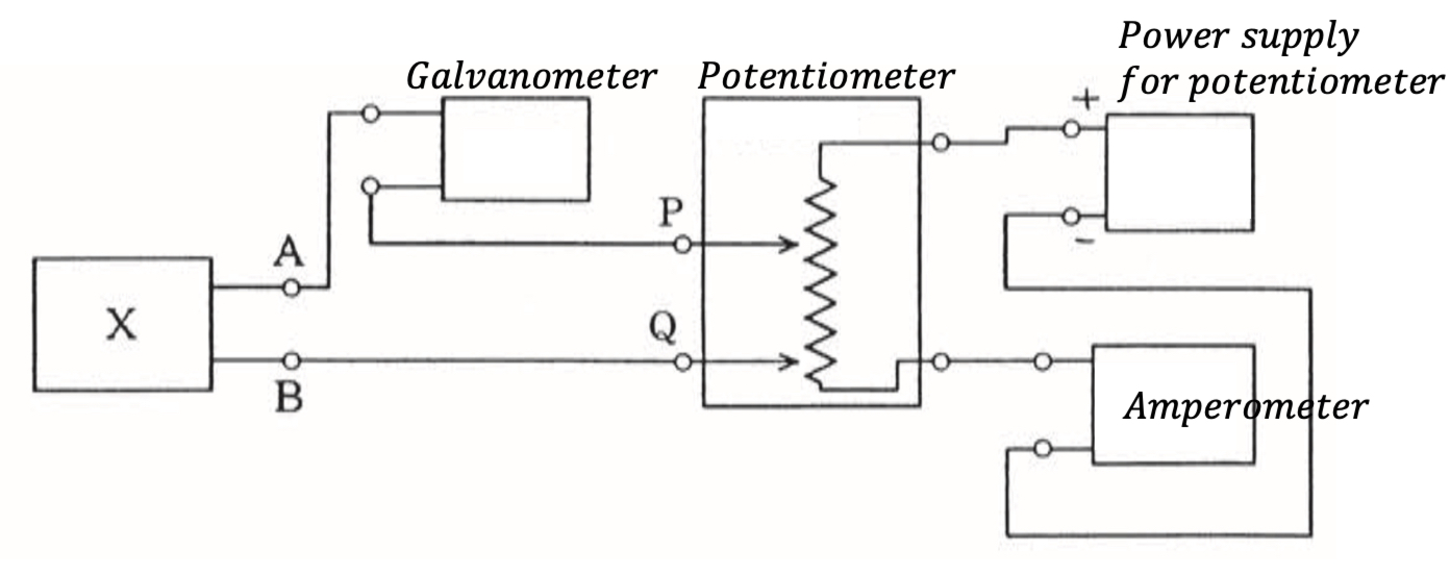
\includegraphics[width=1\linewidth]{figs/Potentiometer_circuit_diagram.pdf}
  \caption{Potentiometer circuit diagram}
  \label{fig:potentiometer}
\end{figure}
まず、$R_{eq}=0$の場合の、端子A、B間の開放端電圧$E_{eq}$を可動コイル型電圧計(3Vレンジ)で測定した。\\
次に、$R_{eq}$を50 $\Omega$から100M $\Omega$まで変化させながら、端子A、B間の開放端電圧$E_{eq}$を可動コイル型電圧計(3Vレンジと10Vレンジ)、エレクトロニクス電圧計、電位差計で測定した。\\
\subsection{テブナンの定理のよる解析値と実測値の比較}
\subsubsection{テブナンの定理を用いた等価電圧と等価抵抗の計算}
図6に実験で解析した回路を示す。
直流安定化電源$E_1[V]$、$E_2[V]$が接続されている。
このモデルの端子\textcircled{1}、\textcircled{2}からみた等価電圧と等価抵抗をテブナンの定理を用いて計算する。
図7に解析の手順を示した。
\begin{figure}[H]
  \centering
  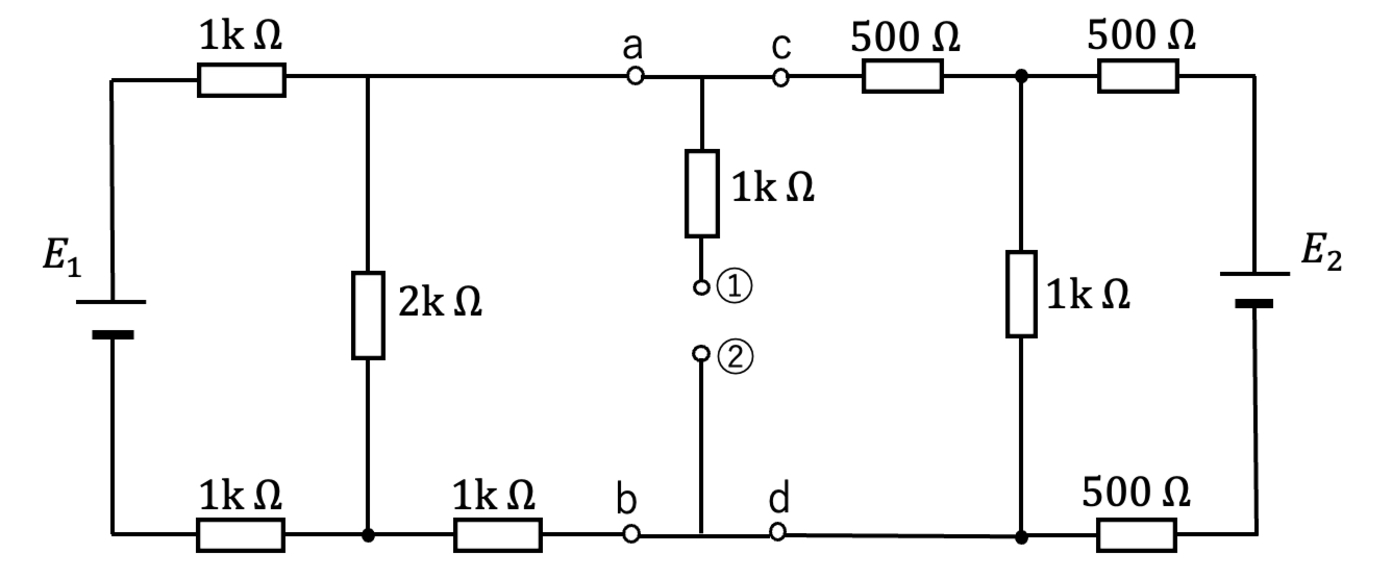
\includegraphics[width=1\linewidth]{figs/circuit_tebnan.pdf}
  \caption{Series Circuit Models}
  \label{fig:tebunan_circuit}
\end{figure}
具体的な手順は以下の通りである:\\
端a-bおよび端c-dで分割する。
まず、端a-bにおける等価回路を求めると、端a-bの回路で、2kΩの抵抗にかかる電圧は$E_1/2$である。また、端a-bから見た抵抗を変化させないことから、端a-bの回路は図5(a)の2段目のように変形できる。
端c-dの回路も同様に変形すると、結果として、端子\textcircled{1}、\textcircled{2}から見た抵抗は
\begin{equation}
R_{eq}=\frac{5\text{k}}{3}\approx 1.667\text{k}[\Omega]
\end{equation}
電圧はKirchhoffの法則を用いて:
\begin{equation}
E_{eq}=\frac{2E_1+E_2}{6} [V]
\end{equation}
と計算される。
\subsubsection{等価電圧$E_{eq}$と等価抵抗$R_{eq}$の測定}
テブナンの定理を用いて計算した電圧(5)式と抵抗値(4)式の値が、実測値と一致するかを確かめた。
以下の手順で開放端電圧と短絡電流を測定し、$E_{eq}$と$R_{eq}$を求めた:

[使用器具]\\
エレクトロニクス直流電圧計 No.2、デジタル電流計 No.3\\

まず、直流電源$E_1$、$E_2$の電圧をエレクトロニクス直流電圧計で測定した。\\
次に、端子\textcircled{1}、\textcircled{2}の開放端電圧をエレクトロニクス直流電圧計で測定した。
その後、端子\textcircled{1}、\textcircled{2}を短絡させ、短絡電流$I_s$をデジタル電流計で測定した。
$R_{eq} = E_{eq}/I_s$より等価抵抗を計算した。\\
\subsubsection{電圧計の$R_m$を変化させた場合の測定}
(3)式より、内部抵抗$R_m$を変数とした場合、開放端電圧$V$は
\begin{equation}
  V(R_m) = \frac{E_{eq}R_m}{R_{eq}+R_m} 
\end{equation}
にプロットされるはずである。このため、以下の手順で$R_m$を変化させた場合の$V$の値を測定した:

[使用器具]\\
エレクトロニクス直流電圧計 No.2、デジタル電流計 No.3、抵抗箱 No.1\\

まず、端子\textcircled{1}、\textcircled{2}間に抵抗箱を接続し、抵抗箱の抵抗値を100 $\Omega$から100k $\Omega$まで変化させた。その際の、開放端電圧$E_{eq}$をエレクトロニクス直流電圧計で測定した。
\end{multicols}

\begin{figure}[H]
  \centering
  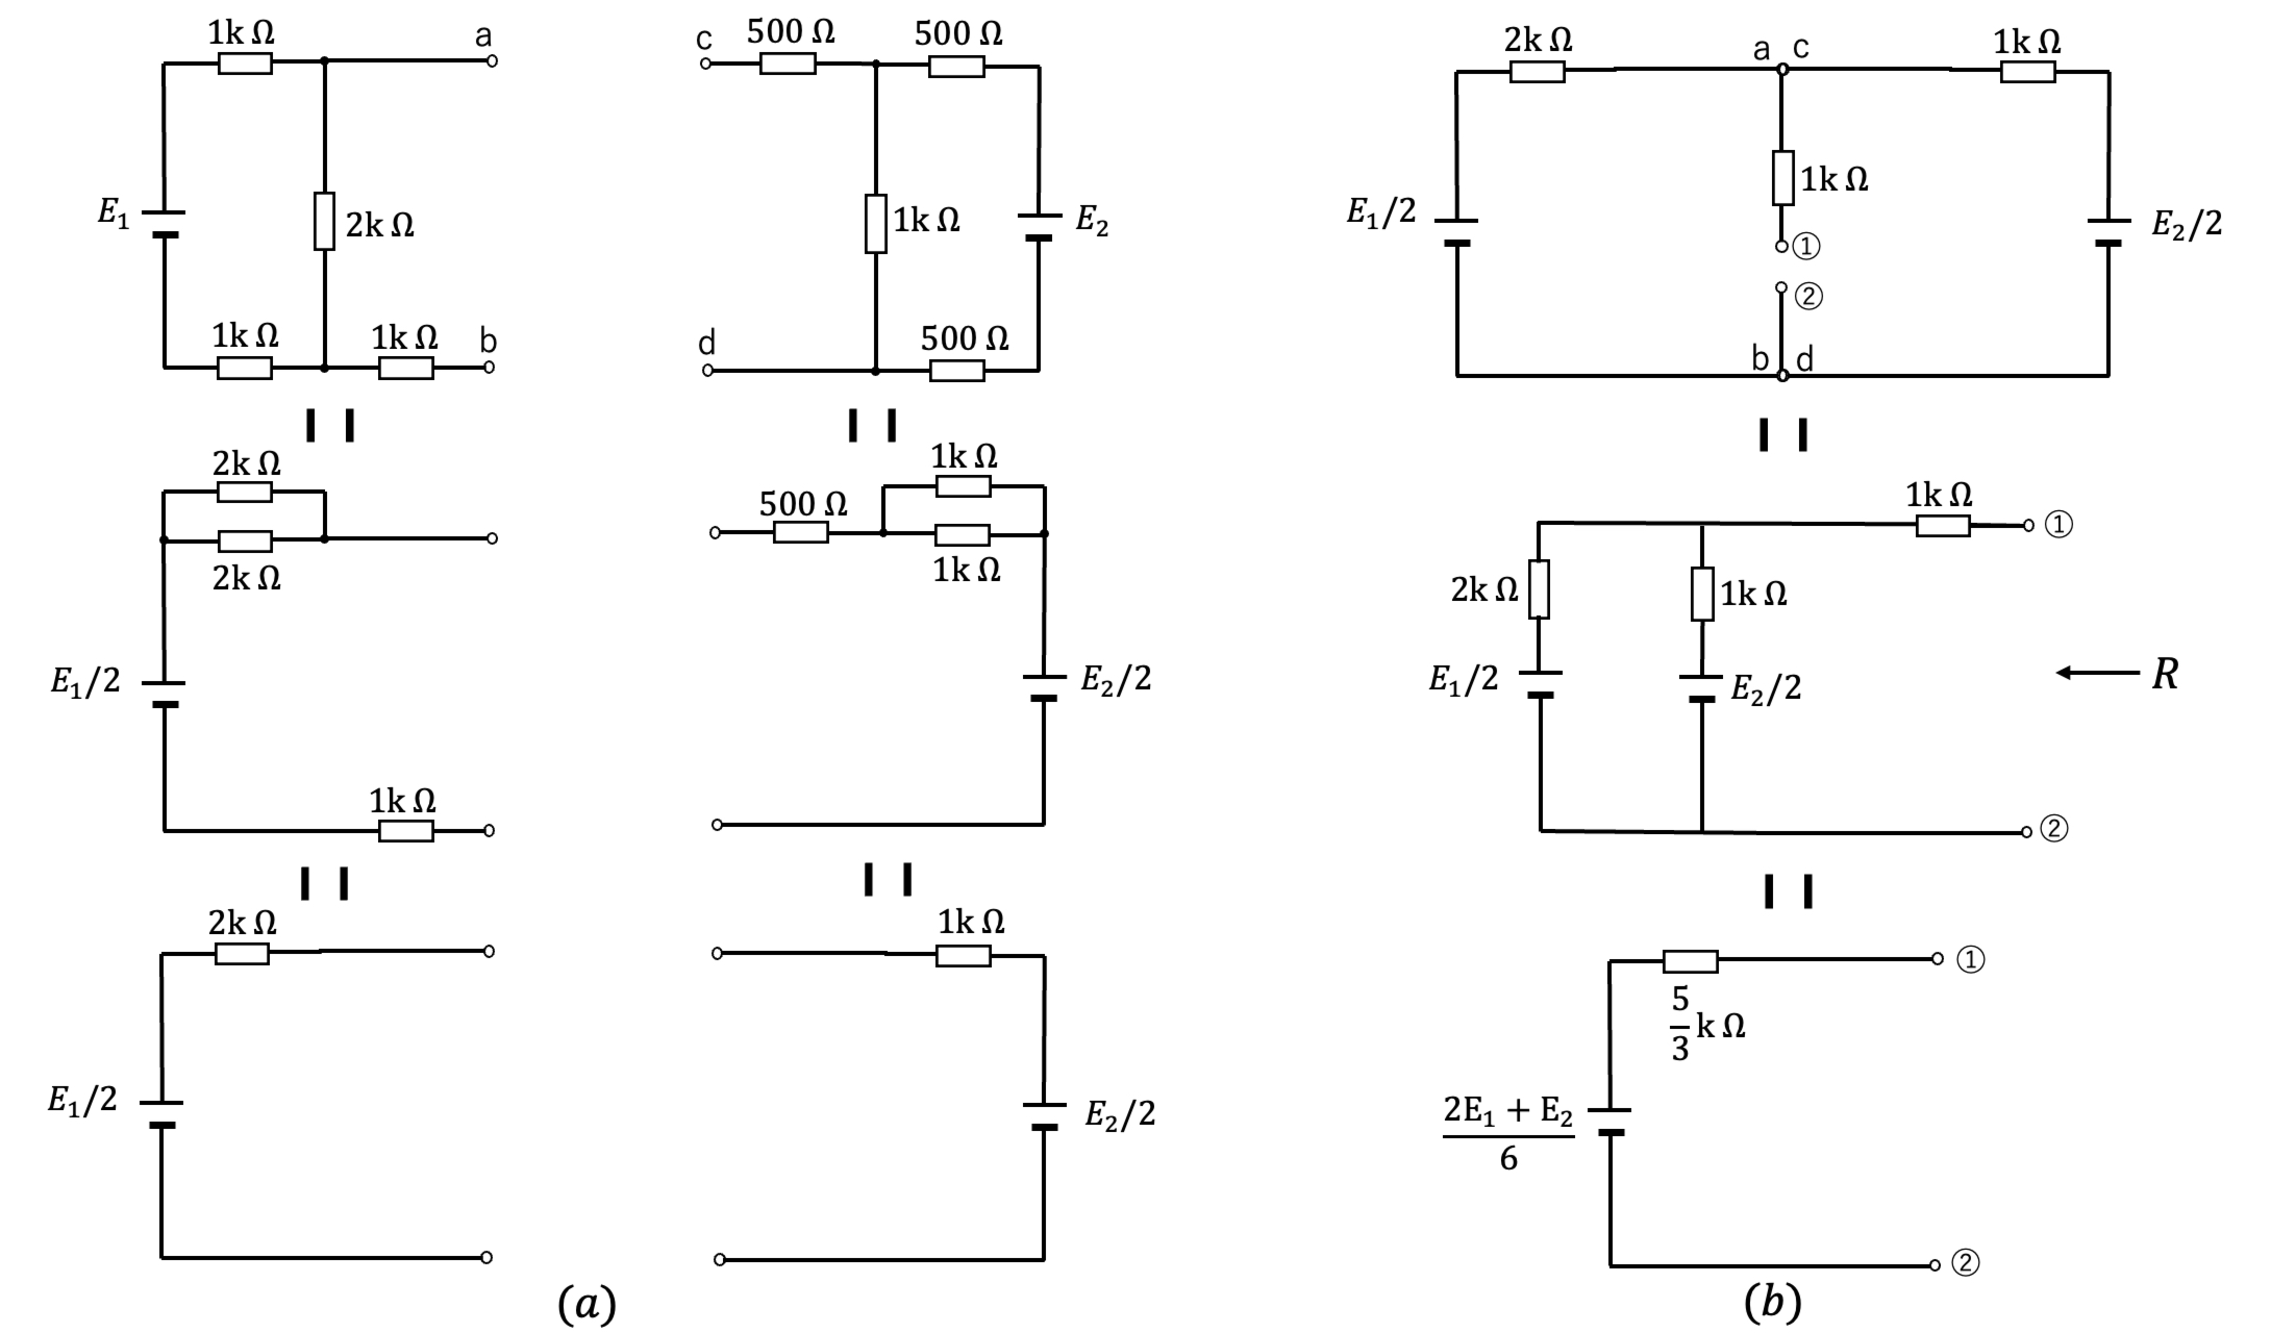
\includegraphics[width=0.8\linewidth]{figs/tebnan_procedure.pdf}
  \caption{Procedure for analyze by Thévenin's Theorem}
  \label{fig:tebnan_procedure}
\end{figure}

\clearpage

\section{Results}
\subsection{開放端電圧の測定結果}
開放端電圧$V$の測定結果を表1に示した。$R_{eq}$は、抵抗箱の抵抗値である。
電位差計では$R_{eq}$が100MΩまで大きくなった場合でも、等価電圧$E_{eq} = 1.550$Vに近い値を測定できていることが分かる。
エレクトロニクス電圧計は、$R_{eq}$が100kΩ程度までならば、安定して等価電圧$E_{eq} = 1.550$Vに近い値を測定できていることが分かる。\\

\begin{table}[htbp]
  \centering
  \caption{Result of V measurement}
    \begin{tabular}{rrrrrrrr}
          &       & \multicolumn{2}{c}{} &       &       &       &  \\
    \multicolumn{1}{l}{$R_{eq}  [\Omega]$} &       & \multicolumn{1}{l}{moving coil (3v range) [V]} & \multicolumn{1}{l}{moving coil (10v range) [V]} &       & \multicolumn{1}{l}{electronics [V]} &       & \multicolumn{1}{l}{potentiometer [V]} \\
    \midrule
    \midrule
    \multicolumn{1}{l}{0} &       & \multicolumn{1}{l}{1.57} &       &       &       &       &  \\
    \multicolumn{1}{l}{50} &       & \multicolumn{1}{l}{1.54} & \multicolumn{1}{l}{1.55} &       & 1.51  &       & 1.5575 \\
    \multicolumn{1}{l}{100} &       & \multicolumn{1}{l}{1.51} & \multicolumn{1}{l}{1.55} &       & 1.51  &       & 1.5575 \\
    \multicolumn{1}{l}{200} &       & \multicolumn{1}{l}{1.47} & \multicolumn{1}{l}{1.55} &       & 1.51  &       & 1.5575 \\
    \multicolumn{1}{l}{500} &       & \multicolumn{1}{l}{1.34} & \multicolumn{1}{l}{1.5} &       & 1.51  &       & 1.5575 \\
    \multicolumn{1}{l}{1k} &       & \multicolumn{1}{l}{1.17} & \multicolumn{1}{l}{1.4} &       & 1.51  &       & 1.5575 \\
    \multicolumn{1}{l}{2k} &       & \multicolumn{1}{l}{0.94} & \multicolumn{1}{l}{1.3} &       & 1.51  &       & 1.5575 \\
    \multicolumn{1}{l}{5k} &       & \multicolumn{1}{l}{0.58} & \multicolumn{1}{l}{1} &       & 1.51  &       & 1.5575 \\
    \multicolumn{1}{l}{10k} &       & \multicolumn{1}{l}{0.36} & \multicolumn{1}{l}{0.8} &       & 1.51  &       & 1.5575 \\
    \multicolumn{1}{l}{20k} &       & \multicolumn{1}{l}{0.2} & \multicolumn{1}{l}{0.5} &       & 1.51  &       & 1.5575 \\
    \multicolumn{1}{l}{50k} &       & \multicolumn{1}{l}{0.08} & \multicolumn{1}{l}{0.25} &       & 1.51  &       & 1.5575 \\
    \multicolumn{1}{l}{100k} &       & \multicolumn{1}{l}{0.04} & \multicolumn{1}{l}{0.15} &       & 1.51  &       & 1.5575 \\
    \multicolumn{1}{l}{200k} &       & \multicolumn{1}{l}{0.02} & \multicolumn{1}{l}{0.1} &       & 1.5   &       & 1.5575 \\
    \multicolumn{1}{l}{500k} &       & \multicolumn{1}{l}{0.01} & \multicolumn{1}{l}{0.05} &       & 1.49  &       & 1.5575 \\
    \multicolumn{1}{l}{1M} &       & \multicolumn{1}{l}{0} & \multicolumn{1}{l}{0} &       & 1.4   &       & 1.5575 \\
    \multicolumn{1}{l}{5M} &       & \multicolumn{1}{l}{0} & \multicolumn{1}{l}{0} &       & 1.2   &       & 1.5575 \\
    \multicolumn{1}{l}{10M} &       & \multicolumn{1}{l}{0} & \multicolumn{1}{l}{0} &       & 0.85  &       & 1.5575 \\
    \multicolumn{1}{l}{20M} &       & \multicolumn{1}{l}{0} & \multicolumn{1}{l}{0} &       & 0.6   &       & 1.5575 \\
    \multicolumn{1}{l}{50M} &       & \multicolumn{1}{l}{0} & \multicolumn{1}{l}{0} &       & 0.4   &       & 1.5575 \\
    \multicolumn{1}{l}{100M} &       & \multicolumn{1}{l}{0} & \multicolumn{1}{l}{0} &       & 0.2   &       & 1.5575 \\
          &       &       &       &       &       &       &  \\
    \end{tabular}%
  \label{tab:addlabel}%
\end{table}%

\begin{figurehere}
  \centering
  \hspace*{2cm}
  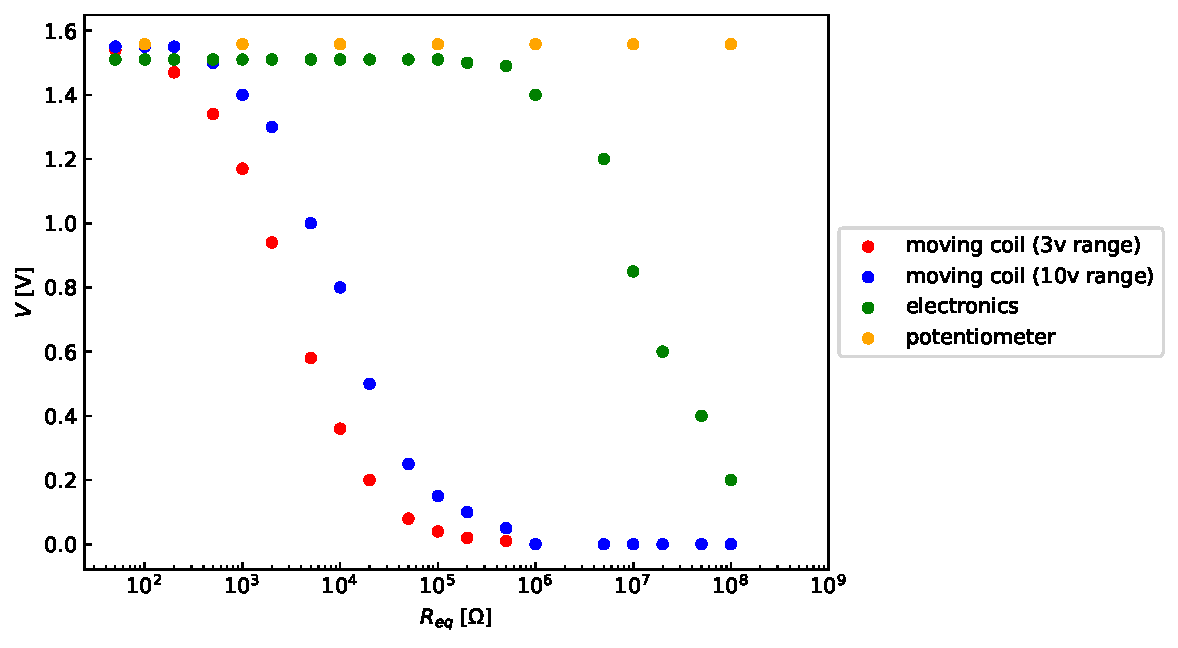
\includegraphics[width=0.75\linewidth]{figs/req_vs_V.pdf}
  \caption{$V$ Plot. \\$R_{eq}$-axis is scaled on a log scale.}
  \label{fig:my_label}
\end{figurehere}


測定点をプロットしたグラフを図8に示した。
x軸は抵抗$R_{eq}$を表しており、対数スケールでプロットしている。y軸は電圧$V$を示している。
電位差計は変化は見られないが、可動コイル型電圧計とエレクトロニクス電圧計は、$R_{eq}$が増加するにつれ$V$が減少しており、$\frac{1}{1 + x}$の関数の特性と一致している。


\subsection{等価電圧$E_{eq}$と等価内部抵抗$R_{eq}$の測定結果}
直流電源の測定結果は、$E_1 = 5.005$ V、$E_2 = 10.055$ Vであった。(5)式に代入すると、$E_{eq} = 3.344$ Vと計算される。
一方、端子\textcircled{1}、\textcircled{2}の開放端電圧$E_{eq}$を測定した結果は、$E_{eq} = 3.31$ Vであった。\\
短絡電流$I_s$を測定した結果は、$I_s = 1.979$ mAであった。従って、$R_{eq} = E_{eq}/I_s$から $1.672$ k$\Omega$と計算される。テブナンの定理による解析値は$1.667$ k$\Omega$であった。
\\いずれも、テブナンの定理による解析値と少数第一位までの二桁の値が一致した。
\subsection{電圧計の$R_m$を変化させた場合の$V$の測定結果}
表2に、$R_m$を100 $\Omega$から100k $\Omega$まで変化させた時の$V$の値の測定結果を示した。
表中の$V_{measured}$は、エレクトロニクス直流電圧計で測定した値、$V_{theoretical}$は、(3)式から計算された値を示している。
(3)式に$E_{eq} = 3.344$ V、$R_{eq} = 1.667$ k$\Omega$を代入すると、$V_{theoretical}$は:
\begin{equation}
  V = \frac{3.344R_m}{1667 + R_m}
\end{equation}
で計算される。
\clearpage 
\begin{table}[htbp]
  \centering
  \caption{Measured and theoretical values of V corresponding to $R_m$}
    \resizebox{0.45\linewidth}{!}{
    \begin{tabular}{rrrrr}
    \multicolumn{1}{l}{$R_m [\Omega]$} &       & \multicolumn{1}{l}{$V_{\text{measured}}$[V]} &       & \multicolumn{1}{l}{$V_{\text{theoretical}}$ [V]} \\
    \midrule
    \midrule
    100   &       & 0.190 &       & 0.189 \\
    200   &       & 0.361 &       & 0.358 \\
    500   &       & 0.752 &       & 0.772 \\
    1000  &       & 1.215 &       & 1.254 \\
    2000  &       & 1.781 &       & 1.824 \\
    5000  &       & 2.511 &       & 2.508 \\
    10000 &       & 2.832 &       & 2.866 \\
    20000 &       & 3.082 &       & 3.087 \\
    50000 &       & 3.201 &       & 3.236 \\
    100000 &       & 3.283 &       & 3.289 \\
    \end{tabular}%
    }
  \label{tab:addlabel}%
\end{table}%

\begin{figure}[htbp]
  \centering
  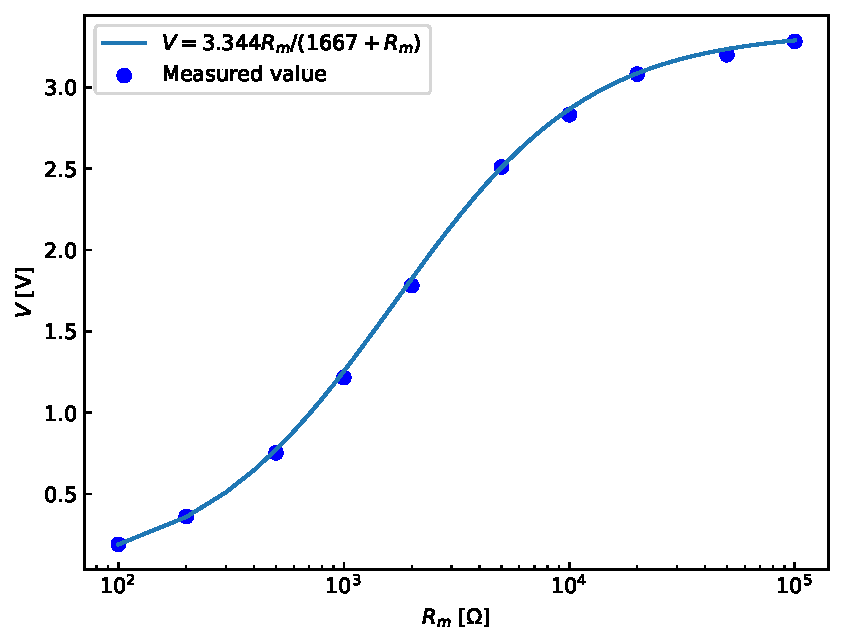
\includegraphics[width=0.6\linewidth]{figs/tebunan.pdf}
  \caption{Relationship between theoretical curves and measured values}
  \label{fig:my_label}
\end{figure}
\vspace{2cm}

図9に、理論曲線(7)式と測定値を同時にプロットしたグラフを示した。
$R_m$は対数目盛で表してある。
プロットされている青色の点は、実際に測定された$V$の値を示している。これらの点は、理論曲線にほぼ従って分布しており、実測値と理論値の一致度は非常に高いことが観察された。
$V = \frac{3.344R_m}{1667 + R_m}$という式で表される理論曲線は、抵抗$R_m$の値が大きくなるにつれて、飽和に向かう形をしており、図9を見ると、$R_m$が100kΩを超えたあたりで$V$の値が飽和していることが確認できる。

\section{Discussion}
\subsection{計器の内部抵抗の計算}
3つの方法で、計器の内部抵抗を求めた。\\\\
方法1:最適にフィットする近似曲線から、$R_m$を導出\\
図8に、最小二乗法より近似曲線$V = \frac{1.55R_m}{R_{eq} + R_m}$をひき、誤差を最小にするときから$R_m$を求めた。
フィッティング結果を図10に示した。
\begin{figure}[H]
  \centering
  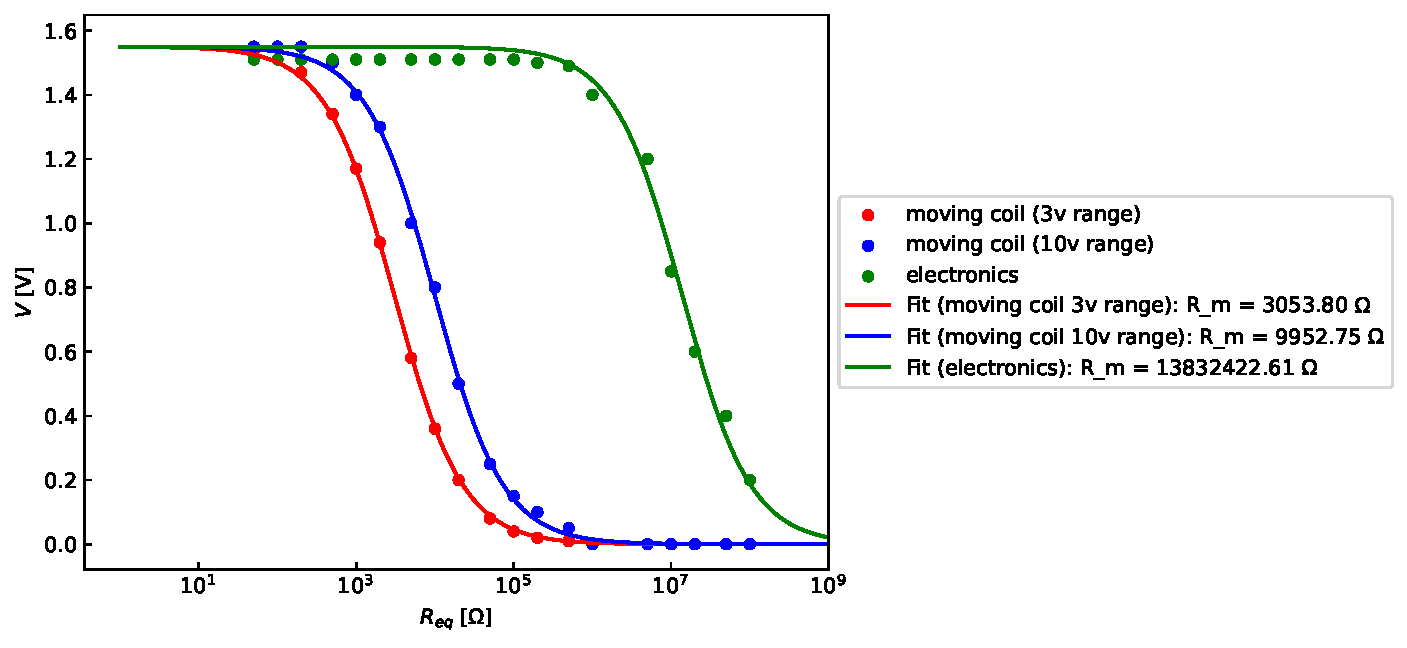
\includegraphics[width=0.9\linewidth]{figs/req-V_fit.pdf}
  \caption{Analyze $R_m$ (Method 1)}
  \label{fig:my_label}
\end{figure}
可動コイル型電圧計(3Vレンジ)、可動コイル型電圧計(10Vレンジ)、エレクトロニクス電圧計の内部抵抗は、それぞれ3.0kΩ、10kΩ、14MΩであった。\\\\
方法2:変曲点付近での線形近似\\
(3)式より、$R_m=R_{eq}$の時、$V=E_{eq}/2$となることから、図8の0.775Vに最も近い2点を取り出して最小二乗法で引いた直線と、$V=0.775$の交点から$R_m$を求めた。\\
変曲点付近で線形近似できる背景としては、(3)式$V = \frac{E_{eq}R_m}{R_{eq}+R_m}$を$R_{eq}=10^x$と変数変換して、Vのxの2回微分が0になる値(変曲点)を求めると、$V=0.775$との交点と非常に近い値になる。\\
最小二乗法で引いた直線と、$V=0.775$を引いたグラフを図11に示した。

\begin{figurehere}
  \centering
  \hspace*{2cm}
  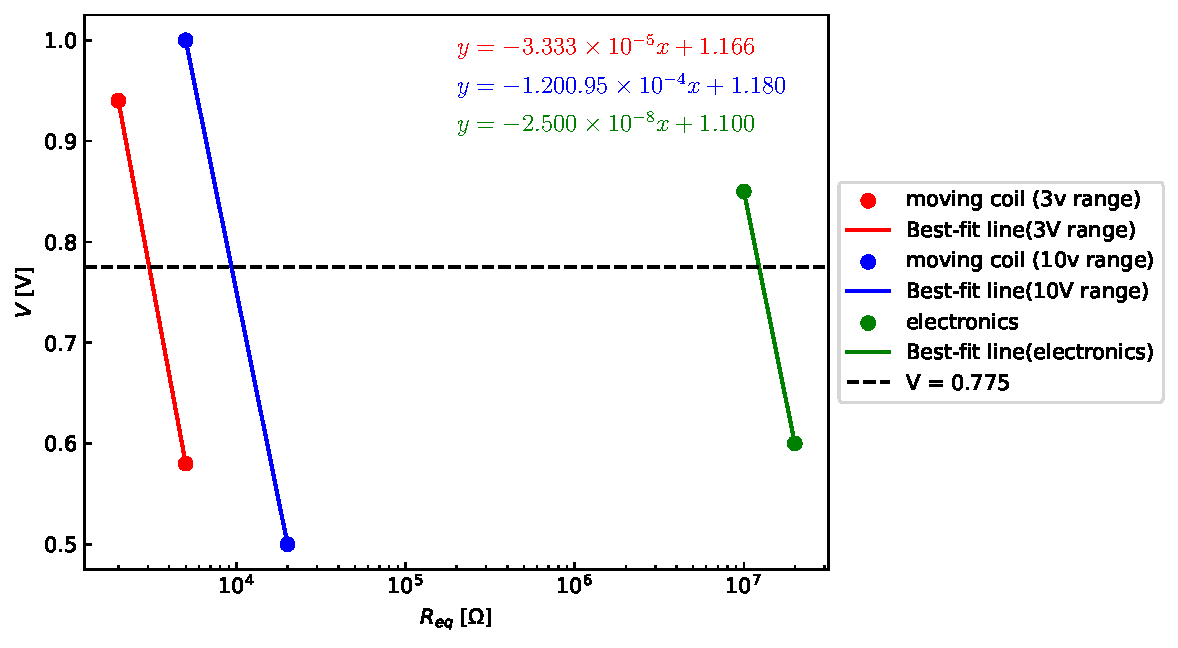
\includegraphics[width=0.7\linewidth]{figs/req_vs_1_V_with_fit_lines.pdf}
  \caption{Analyze $R_m$ (Method 2)}
  \label{fig:my_label}
\end{figurehere}
交点から、$R_{m}$を求めた結果を表3に示した。
\begin{table}[H]
  \centering
  \caption{Results of $R_m$ calculation by Method 1}
    \begin{tabular}{ll}
          & \multicolumn{1}{l}{$R_m$ [Ω]} \\
    \midrule
    \midrule
    moving coil (3v range) & 3.3k \\
    moving coil (10v range) & 11k \\
    electronics & 13M \\
    \end{tabular}%
  \label{tab:addlabel}%
\end{table}%\\\\
方法3: 縦軸$1/V$として重み付き最小二乗法の傾きから導出
(3)式を変形すると:
\begin{equation}
  \frac{1}{V} = \frac{1}{E_{eq}} + \frac{R_{eq}}{E_{eq}R_m}
\end{equation}
となるので、$1/V$を縦軸、$R_{eq}$を横軸として直線を引いた際の傾きから$R_m$を求めることができる。\\
プロットした点から重み付き最小二乗法で直線を引いた。その結果を図12に示した。\\

\begin{figure}[H]
  \hspace*{2cm}
  \centering
  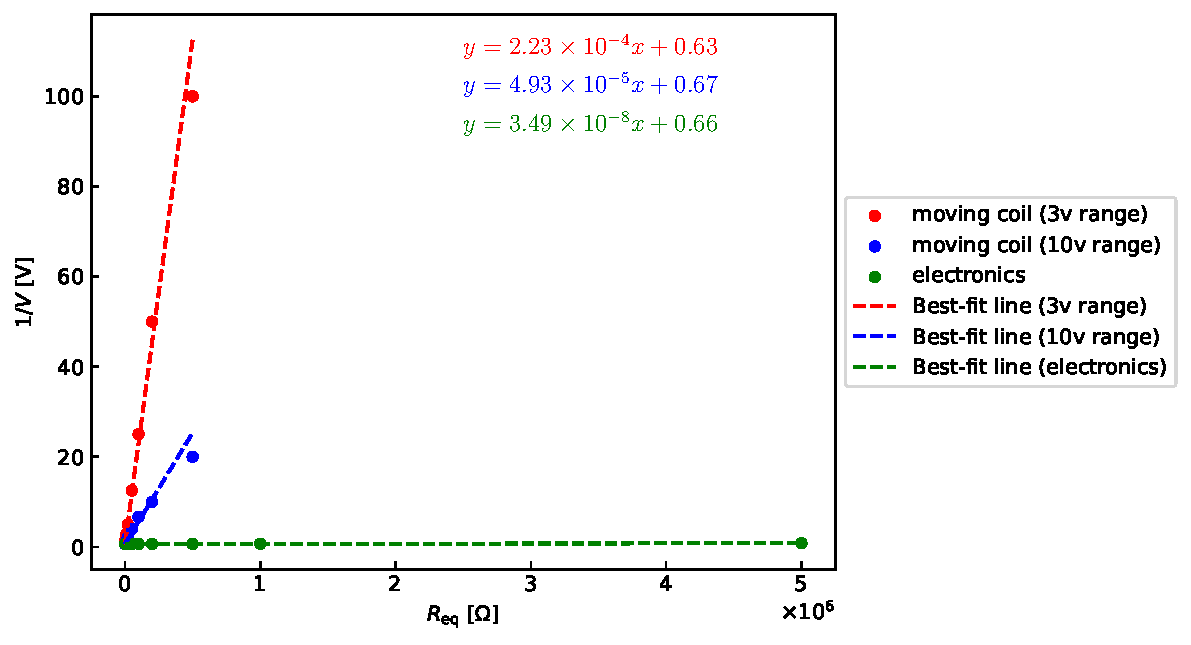
\includegraphics[width=0.7\linewidth]{figs/req_vs_V_with_fit_lines.pdf}
  \caption{Analyze $R_m$ (Method 2)}
  \label{fig:my_label}
\end{figure}

近似曲線の切片は、いずれも$1/E_{eq} = 0.645$に近い値をとっている。\\
それぞれの電圧計において得られた直線の傾きから、$R_m$を求めた。
表4に、その結果を示した。
% Table generated by Excel2LaTeX from sheet 'tex'
\begin{table}[H]
  \centering
  \caption{Results of $R_m$ calculation by Method 2}
    \begin{tabular}{ll}
          & $R_m$ [Ω] \\
    \midrule
    \midrule
    moving coil (3v range) & 2.8k \\
    moving coil (10v range) & 13k \\
    electronics &  18M \\
    \end{tabular}%
  \label{tab:addlabel}%
\end{table}%

\section{Conclusion}

可動コイル型電圧計は、測定対象の電圧変化を非常に高い精度で検出できる。今回用いた可動コイル型電圧計の場合、$R_{eq}$が100Ω程度であれば、可動コイル型電圧計を用いることで$V$は$E_{eq}$に非常に近い値をとることできる。しかし、可動コイル型電圧計の内部抵抗は小さかったため、$R_{eq}$が非常に大きい場合は、電位差計を用いると$V$は$E_{eq}$に近い値を測定することができる。
一方で、エレクトロニクス電圧計は、可動コイル型電圧計に比べて内部抵抗が大きかったため、$R_{eq}$が10kΩ程度であれば、$E_{eq}$に近い値を測定することができた。

\begin{thebibliography}{文献数}
\bibitem{ID} 東京理科大学理学部応用物理学科, ``物理学実験テキスト'', 2023.
\end{thebibliography}
\clearpage

\end{document}